% !TeX root = ../main.tex

\section{Introduction}
\frame{\sectionpage}

\begin{frame}{Social Distancing under Pandemic}
  \begin{itemize}
    \item Social distancing measures
    \begin{columns}[c]  %开始进入分栏环境,居中设置
      \column{6cm}  %第一栏(左栏)宽度为5cm
      \begin{figure}[ht]
        \centering
        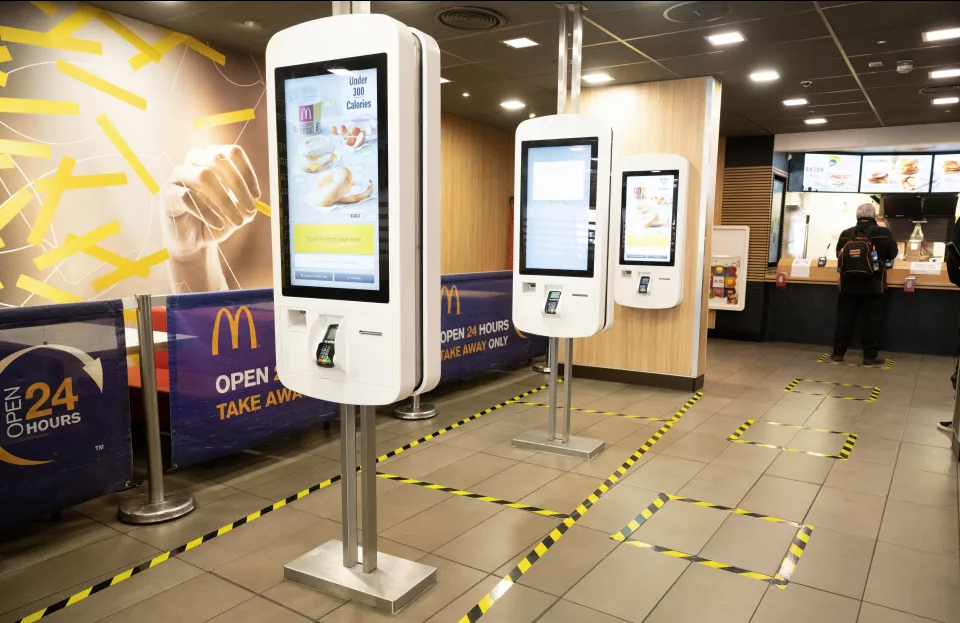
\includegraphics[width = 0.7\textwidth]{./images/McDonald.png}
        % \caption{Problem Conversion with One Seat as Social Distancing}
      \end{figure}
      \column{4cm}
      \scriptsize
      \begin{figure}[ht]
        \centering
        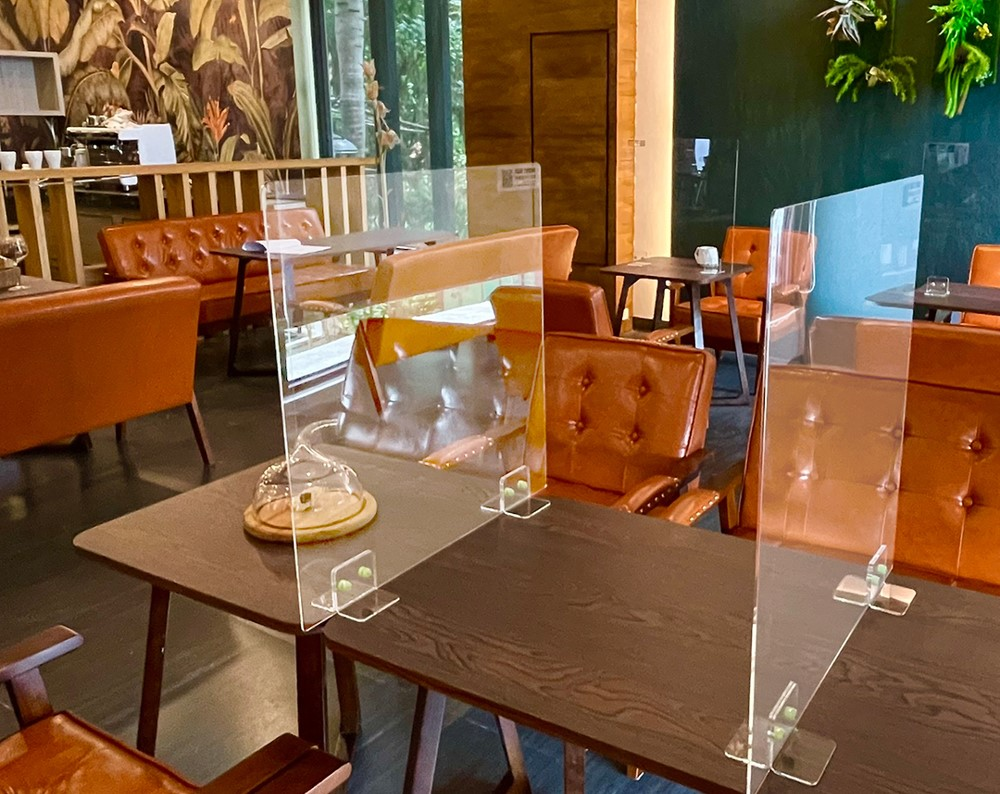
\includegraphics[width=0.9\textwidth,height=0.7\textwidth]{./images/res2.jpg}
        % \caption{Problem Conversion with One Seat as Social Distancing}
      \end{figure}
      \end{columns} 

      \begin{columns}[c]  %开始进入分栏环境,居中设置
        \column{5.5cm}  %第一栏(左栏)宽度为5cm
        \begin{figure}[ht]
          \centering
          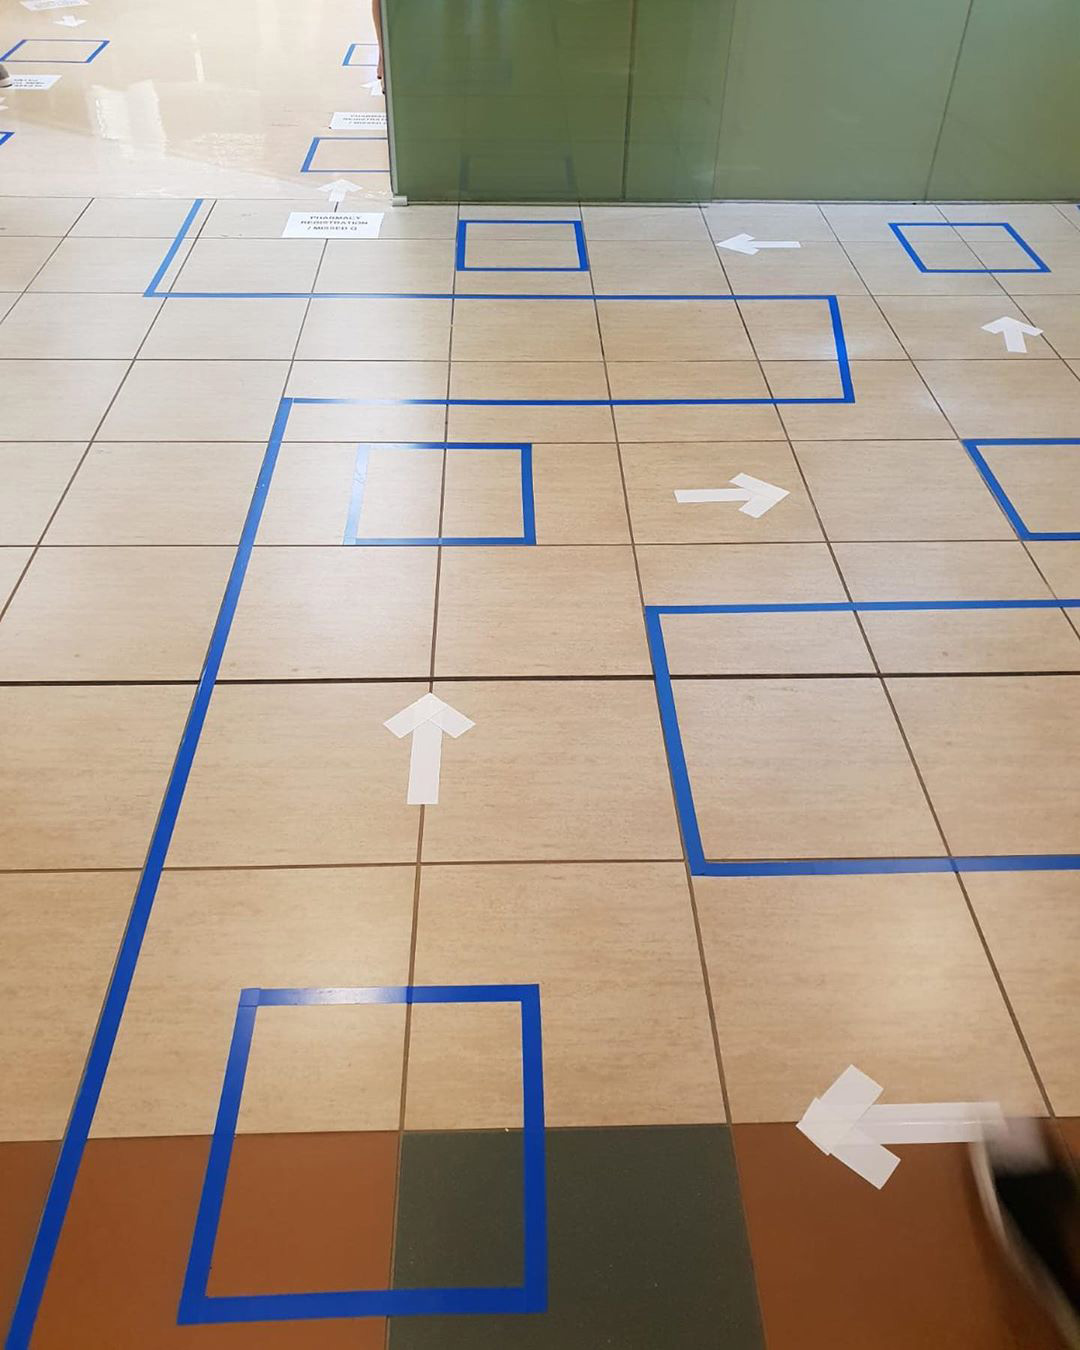
\includegraphics[width = 0.7\textwidth, height=0.5\textwidth]{./images/social_distancie_tape.jpg}
        \end{figure}
        \column{4.5cm}
        \scriptsize
        \begin{figure}[ht]
          \centering
          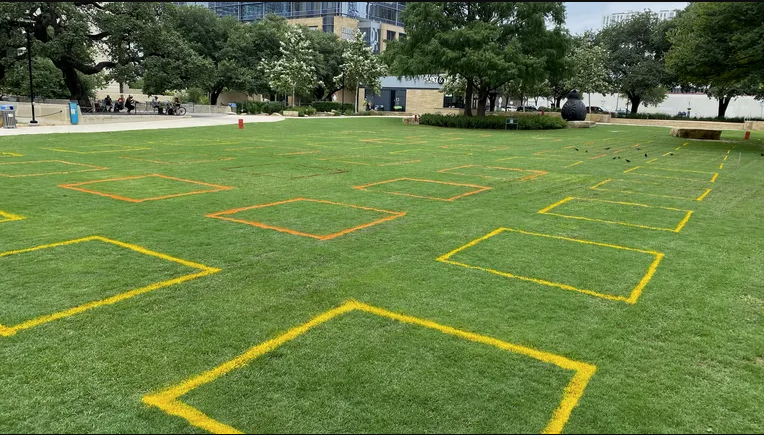
\includegraphics[width = 0.9\textwidth]{./images/socail_park.png}
        \end{figure}
        \end{columns} 
  \end{itemize}
  \end{frame}


  \begin{frame}{Social Distancing under Pandemic}
    \begin{itemize}
      \item Social distancing in seating areas
      \begin{columns}[c]  %开始进入分栏环境,居中设置
        \column{5cm}  %第一栏(左栏)宽度为5cm
        \begin{figure}[ht]
          \centering
          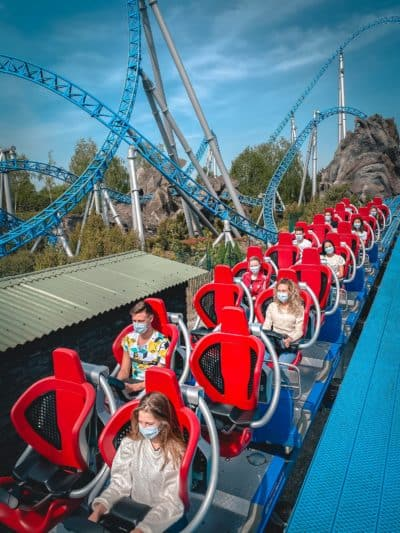
\includegraphics[width = 0.8\textwidth, height=0.6\textwidth]{./images/park_social_distancing.jpg}

        \end{figure}
        \column{5cm}
        \scriptsize
        \begin{figure}[ht]
          \centering
          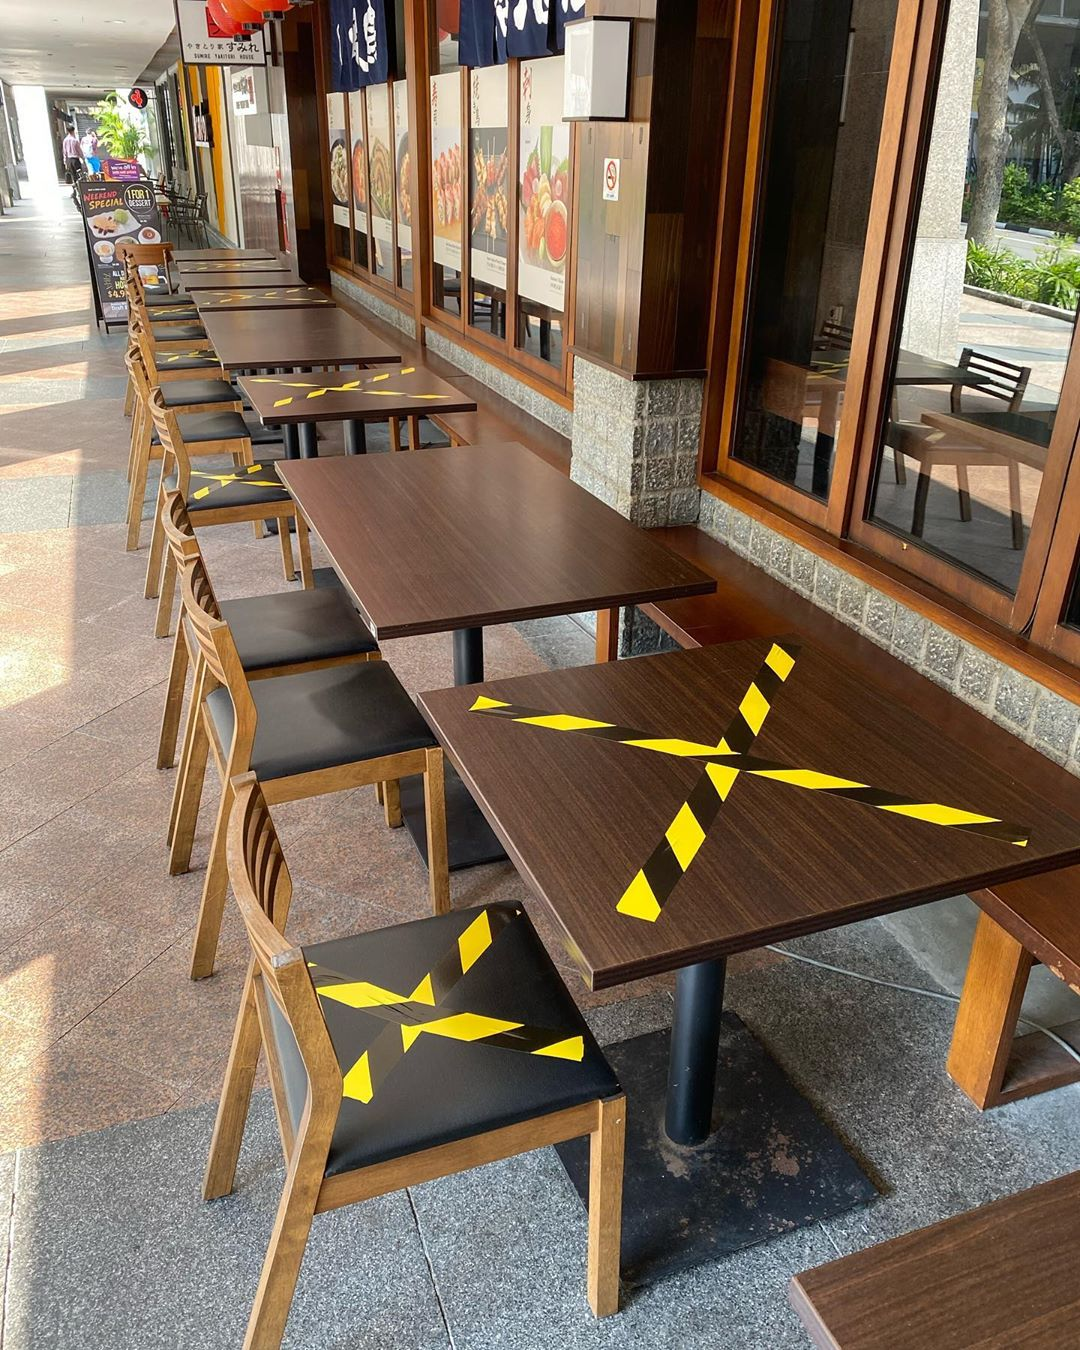
\includegraphics[width=0.8\textwidth,height=0.6\textwidth]{./images/tape_measures.jpg}
        \end{figure}

        \end{columns} 
        
        \begin{columns}[c]  %开始进入分栏环境,居中设置
          \column{5cm}  %第一栏(左栏)宽度为5cm
          \begin{figure}[ht]
            \centering
            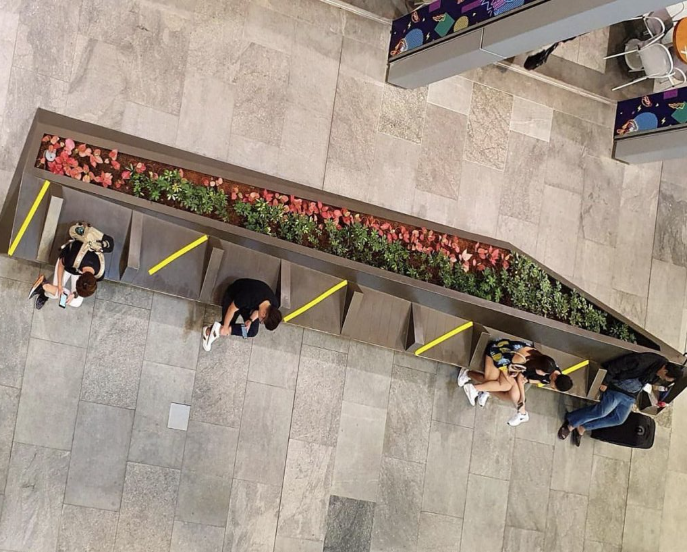
\includegraphics[width = 0.8\textwidth]{./images/seat_sc.png}
          \end{figure}
          \column{5cm}
          \scriptsize
          \begin{figure}[ht]
            \centering
            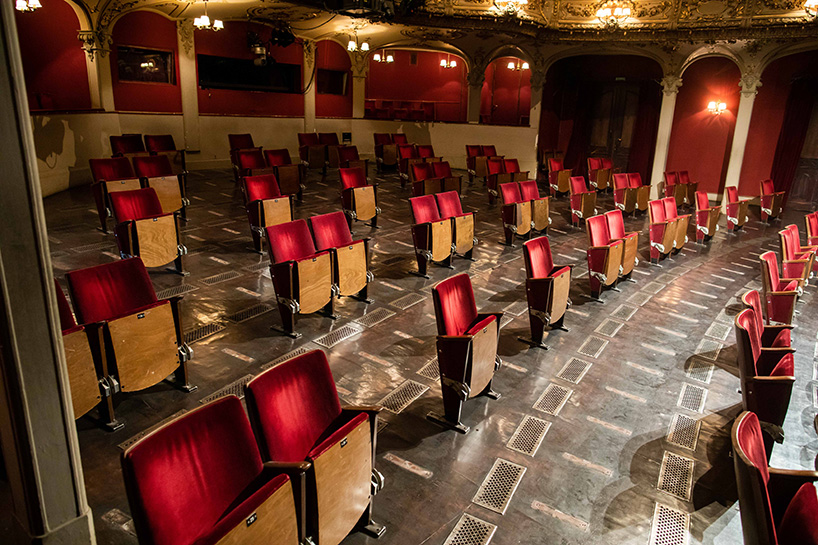
\includegraphics[width = 0.9\textwidth]{./images/cinema.jpg}
          \end{figure}
          \end{columns} 
    \end{itemize}
    \end{frame}

    \begin{frame}{Seat Planning And Seat Assignment}
      There is a requirement for the maximum number of people in one group.
      
      People in one group should sit together.
      
      \vspace{1cm}

      \begin{columns}
        \column{5cm}  %第一栏(左栏)宽度为5cm
        Seat planning: 
          \begin{figure}[ht]
            \centering
            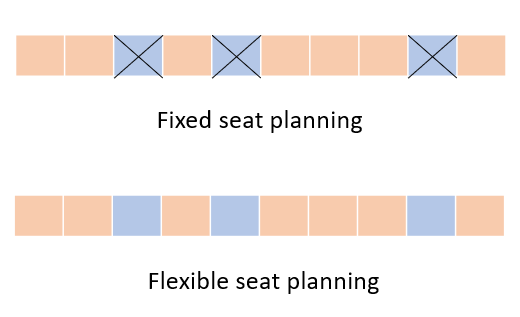
\includegraphics[width = 0.8\textwidth]{./images/seat_planning.png}
          \end{figure}
          \column{5cm}
        Seat assignment: 
          \scriptsize
          \begin{figure}[ht]
            \centering
            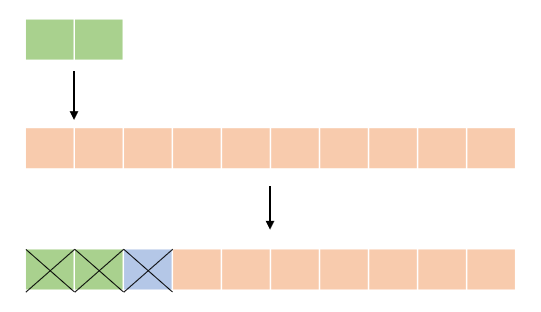
\includegraphics[width = 0.8\textwidth]{./images/seat_assignment.png}
          \end{figure}
      \end{columns}
    
    \end{frame}
    

    \begin{frame}{Situations}
      \begin{itemize}
        \item Deterministic Demand
        
        Make the seat planning with the known specific demand for each group.
        \item Stochastic Demand
        
        Make the seat planning with the known demand distribution before the demand realization.
            
        \item Dynamic Demand

        1. Assign seats to each group under fixed seat planning.

        2. Assign seats to each group.
        
        2.1: Assign seats to each group after its realization.
    
        2.2: Accept or reject each group after its realization, but assign them later.
    
      \end{itemize}
    \end{frame}